\section{Ergebnisse}
\label{sec:Ergebnisse}

Nachdem beide Methoden trainiert wurden, wurden die so entstandenen Modelle evaluiert.
In \autoref{tab:accuracy} sind alle erreichten Genauigkeiten aufgelistet.

\begin{table}
    \centering
    \caption{Genauigkeit der verwendeten Methoden auf den verschiedenen Teildatensätzen, wobei mit CNN das Convolutional Neural Network gemeint ist}
    \label{tab:accuracy}
    \resizebox*{0.8\textwidth}{!}{%
    \begin{tabular}{l c c c}
        \toprule 
        Methode & Trainingsdaten & Validierungsdaten & Testdaten \\ 
        \midrule 
        CNN (standard Schwellwert 0,50) & 93,56\% & 93,05\% & 93,30\% \\
        CNN (bester Schwellwert 0,54) & 93,58\% & 93,07\% & 93,32\% \\
        Random Forest & 89,40\% & 89,09\% & 89,37\% \\
        \bottomrule
    \end{tabular}%
    }
\end{table}

Hier ist deutlich zu erkennen, dass beide von uns gewählten Methoden gute Ergebnisse erzielten, jedoch die Hauptmethode eine deutlich höhere Genauigkeit erzielte.
Eine genauere Analyse der Ergebnisse ist über eine Konfusionsmatrix erreichbar und diese ist in \autoref{fig:confusionmatrix} dargestellt.

\begin{figure}
    \centering
    \begin{subfigure}{0.4\textwidth}
        \centering
        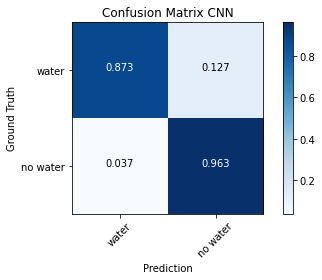
\includegraphics[width=\textwidth]{images/cm_cnn.png}
        \caption{Hauptmethode}
        \label{fig:cm_cnn}
    \end{subfigure}
    \begin{subfigure}{0.4\textwidth}
        \centering
        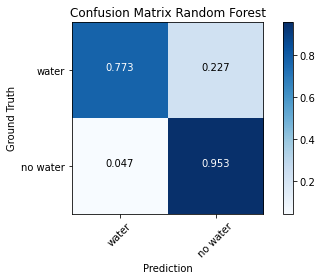
\includegraphics[width=\textwidth]{images/cm_rndf.png}
        \caption{Alternativmethode}
        \label{fig:cm_rndf}
    \end{subfigure}
    \caption{Konfusionsmatrizen der Vorhersagen der verwendeten Methoden auf dem Testdatensatz}
    \label{fig:confusionmatrix}
\end{figure}

Um die Methoden allerdings tatsächlich evaluieren zu können ist es notwendig einige Beispiele der vorhergesagten Masken zu betrachten.
Dazu ist in \autoref{fig:beispiele_cnn} die Ausgabe des Convolutional Neural Network mit und ohne binäre Darstellung mittels des Schwellwertes dargestellt.
Außerdem ist in \autoref{fig:beispiele_rndf} die zusätzliche Eingabe des Gradienten des Satellitenbildes und die Ausgabe des Random Forest zu sehen.

\begin{figure}
    \centering
    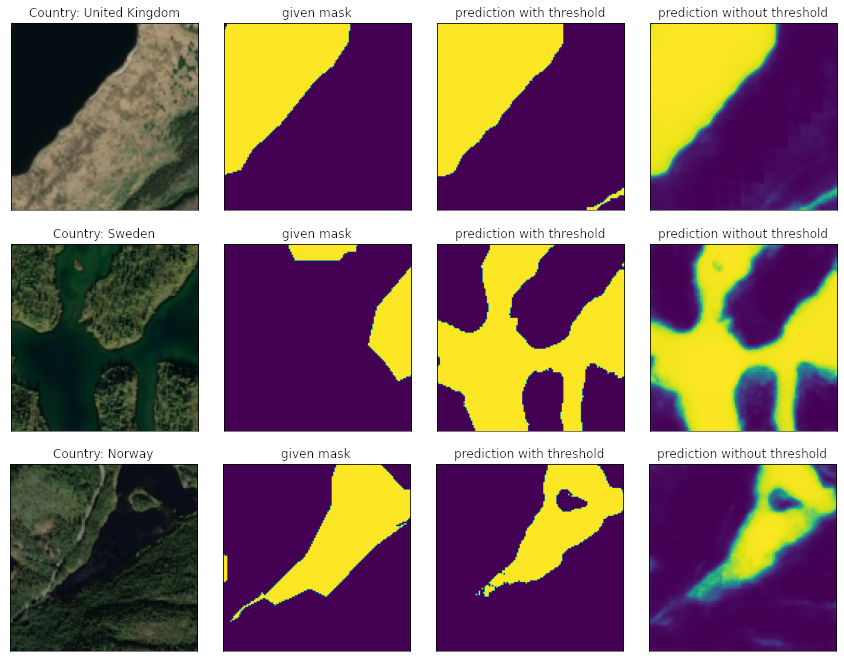
\includegraphics[width=0.8\textwidth]{images/bsp_cnn.png}
    \caption{Beispiele der Vorhersagen des Convolutional Neural Network mit und ohne Anwendung des Schwellwertes. %
    \\ \copyright Mapbox, \copyright OpenStreetMap}
    \label{fig:beispiele_cnn}
\end{figure}

\begin{figure}
    \centering
    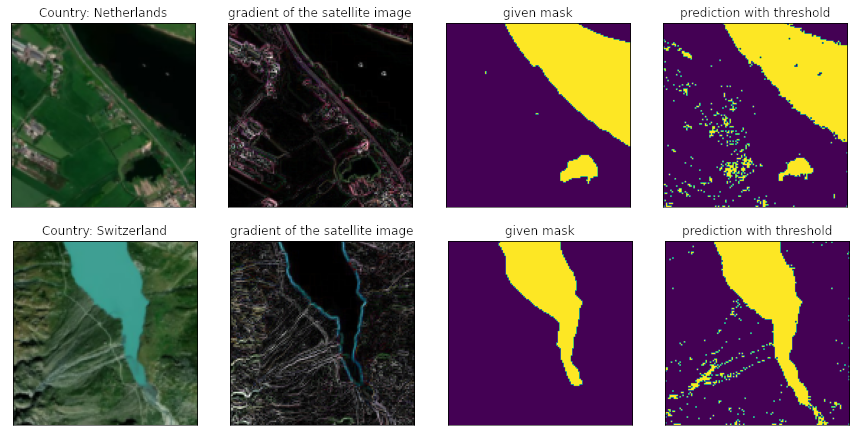
\includegraphics[width=0.8\textwidth]{images/bsp_rndf.png}
    \caption{Beispiele der Vorhersagen des Random Forest und  %
    das Bild der Gradienten des Satellitenbildes. %
    \\ \copyright Mapbox, \copyright OpenStreetMap}
    \label{fig:beispiele_rndf}
\end{figure}

Schon hier lässt sich erkennen, dass die Alternativmethode deutlich mehr Rauschen aufgrund der pixelweisen Klassifizierung erzeugte.
Die Hauptmethode konnte nicht alle Pixel eindeutig zuordnen und vor Allem Ränder oder schwer zu klassifizierende Stellen erhielten Werte die eher mittig zwischen 0 und 1 liegen.
Auch ist schon zu sehen, dass die gegebene Maske nicht perfekt war und teilweise Gewässer gar nicht oder nur grob markiert waren.

Um weitere Erkenntnisse zu den beiden Methoden zu bekommen, werden in \autoref{fig:vergleich} die Vorhersagen beider Methoden miteinander verglichen.
Weitere Beispiele sind im Anhang in \autoref{fig:bsp} und in \autoref{fig:bsp_bad} dargestellt.

\begin{figure}
    \centering
    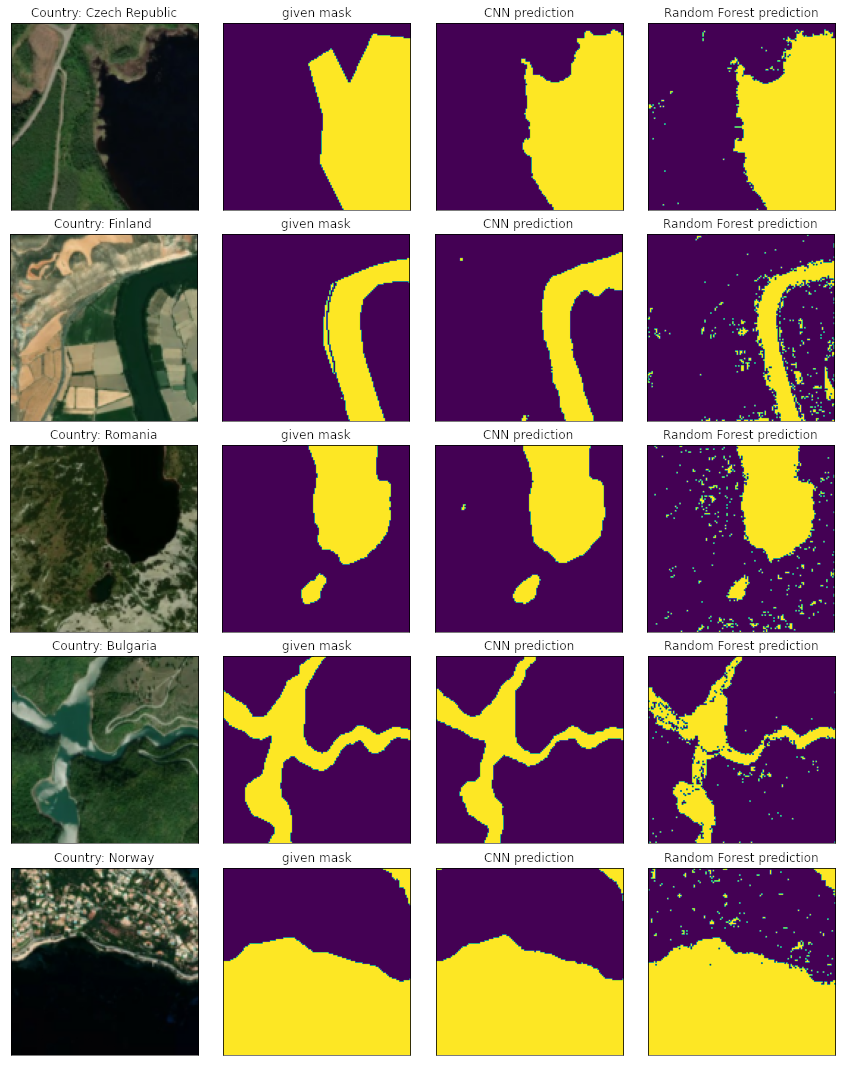
\includegraphics[width=0.9\textwidth]{images/vergleich.png}
    \caption{Beispiele zum Vergleich der Hauptmethode zur Alternativmethode. %
    Aufgezeigt sind (von rechts nach links) das Satellitenbild, die Maske im Datensatz, die Vorhersage des Convolutional Neural Network und die Vorhersage des Random Forest.%
    \\ \copyright Mapbox, \copyright OpenStreetMap}
    \label{fig:vergleich}
\end{figure}

Häufig ist die gegebene Maske nicht sehr detailliert 
und obwohl beide Modelle auf diesen fehlerhaften Daten trainiert wurden,
wurden die Grenzen der Gewässer häufig klar erkannt.
Aufgrund dieser fehlerhaften gegebenen Masken war auch eine Genauigkeit von 100\% nicht erreichbar.

In \autoref{fig:bsp_bad} sind zusätzlich noch einige Beispiele aufgezeigt, 
bei denen die Segmentierung nicht gut funktionierte 
oder die gegebene Maske falsch war.
Probleme waren z.B. Wolken, Ebbe und Flut, Felder, Sumpfgebiete, Schnee oder sonstige auch für den Menschen schwer zu erkennende Gewässer.
Um tatsächlich alle Probleme sehen zu können, müssten deutlich mehr Bilder gezeigt werden, dies würde allerdings den Rahmen dieses Berichtes sprengen.
Teilweise ist nicht erklärbar warum die Algorithmen Wasser falsch erkannten.
Häufig entstanden Fehler an Stellen, die auch ein Mensch nicht erkennen könnte, aber manchmal wurden selbst eindeutige Kanten nicht richtig erkannt.
Einige der Fehler waren sicherlich auf die niedrige Auflösung von 128x128 Pixel zurückzuführen, aber die meisten Gewässer waren auch mit dieser Auflösung klar zu erkennen.
